In this adaptive strategy, the VMS-based error is calculated on the initial mesh. Based on the estimated error, a nodal size field is calculated using the Equation \eqref{eq:diez}, see Section \ref{sec:sf_adapt}.

% \begin{equation}
% \frac{e_k}{\tilde{e}_k} = \left(\frac{h_{old}}{h_{new}}\right)^{m+N/2} 
% \label{eq:diez}
% \end{equation}

%Here, $e_k$ is the measured local error (in the $\HOne$-seminorm) at an element $k$, $\tilde{e}_k$ is the target error for an element specified by the user, $m$ is the polynomial order of the approximation space (i.e., $m=1$ for the linear finite elements used currently) , and $N$ is the number of spatial dimensions. $h_{old}$ is current size of the element, and $h_{new}$ is the desired new mesh size.
%This new mesh size at the element level is assembled at the node/vertex level to perform mesh adaptation.

\begin{figure}[H]
\centering
\begin{subfigure}[b]{0.475\textwidth}
\centering
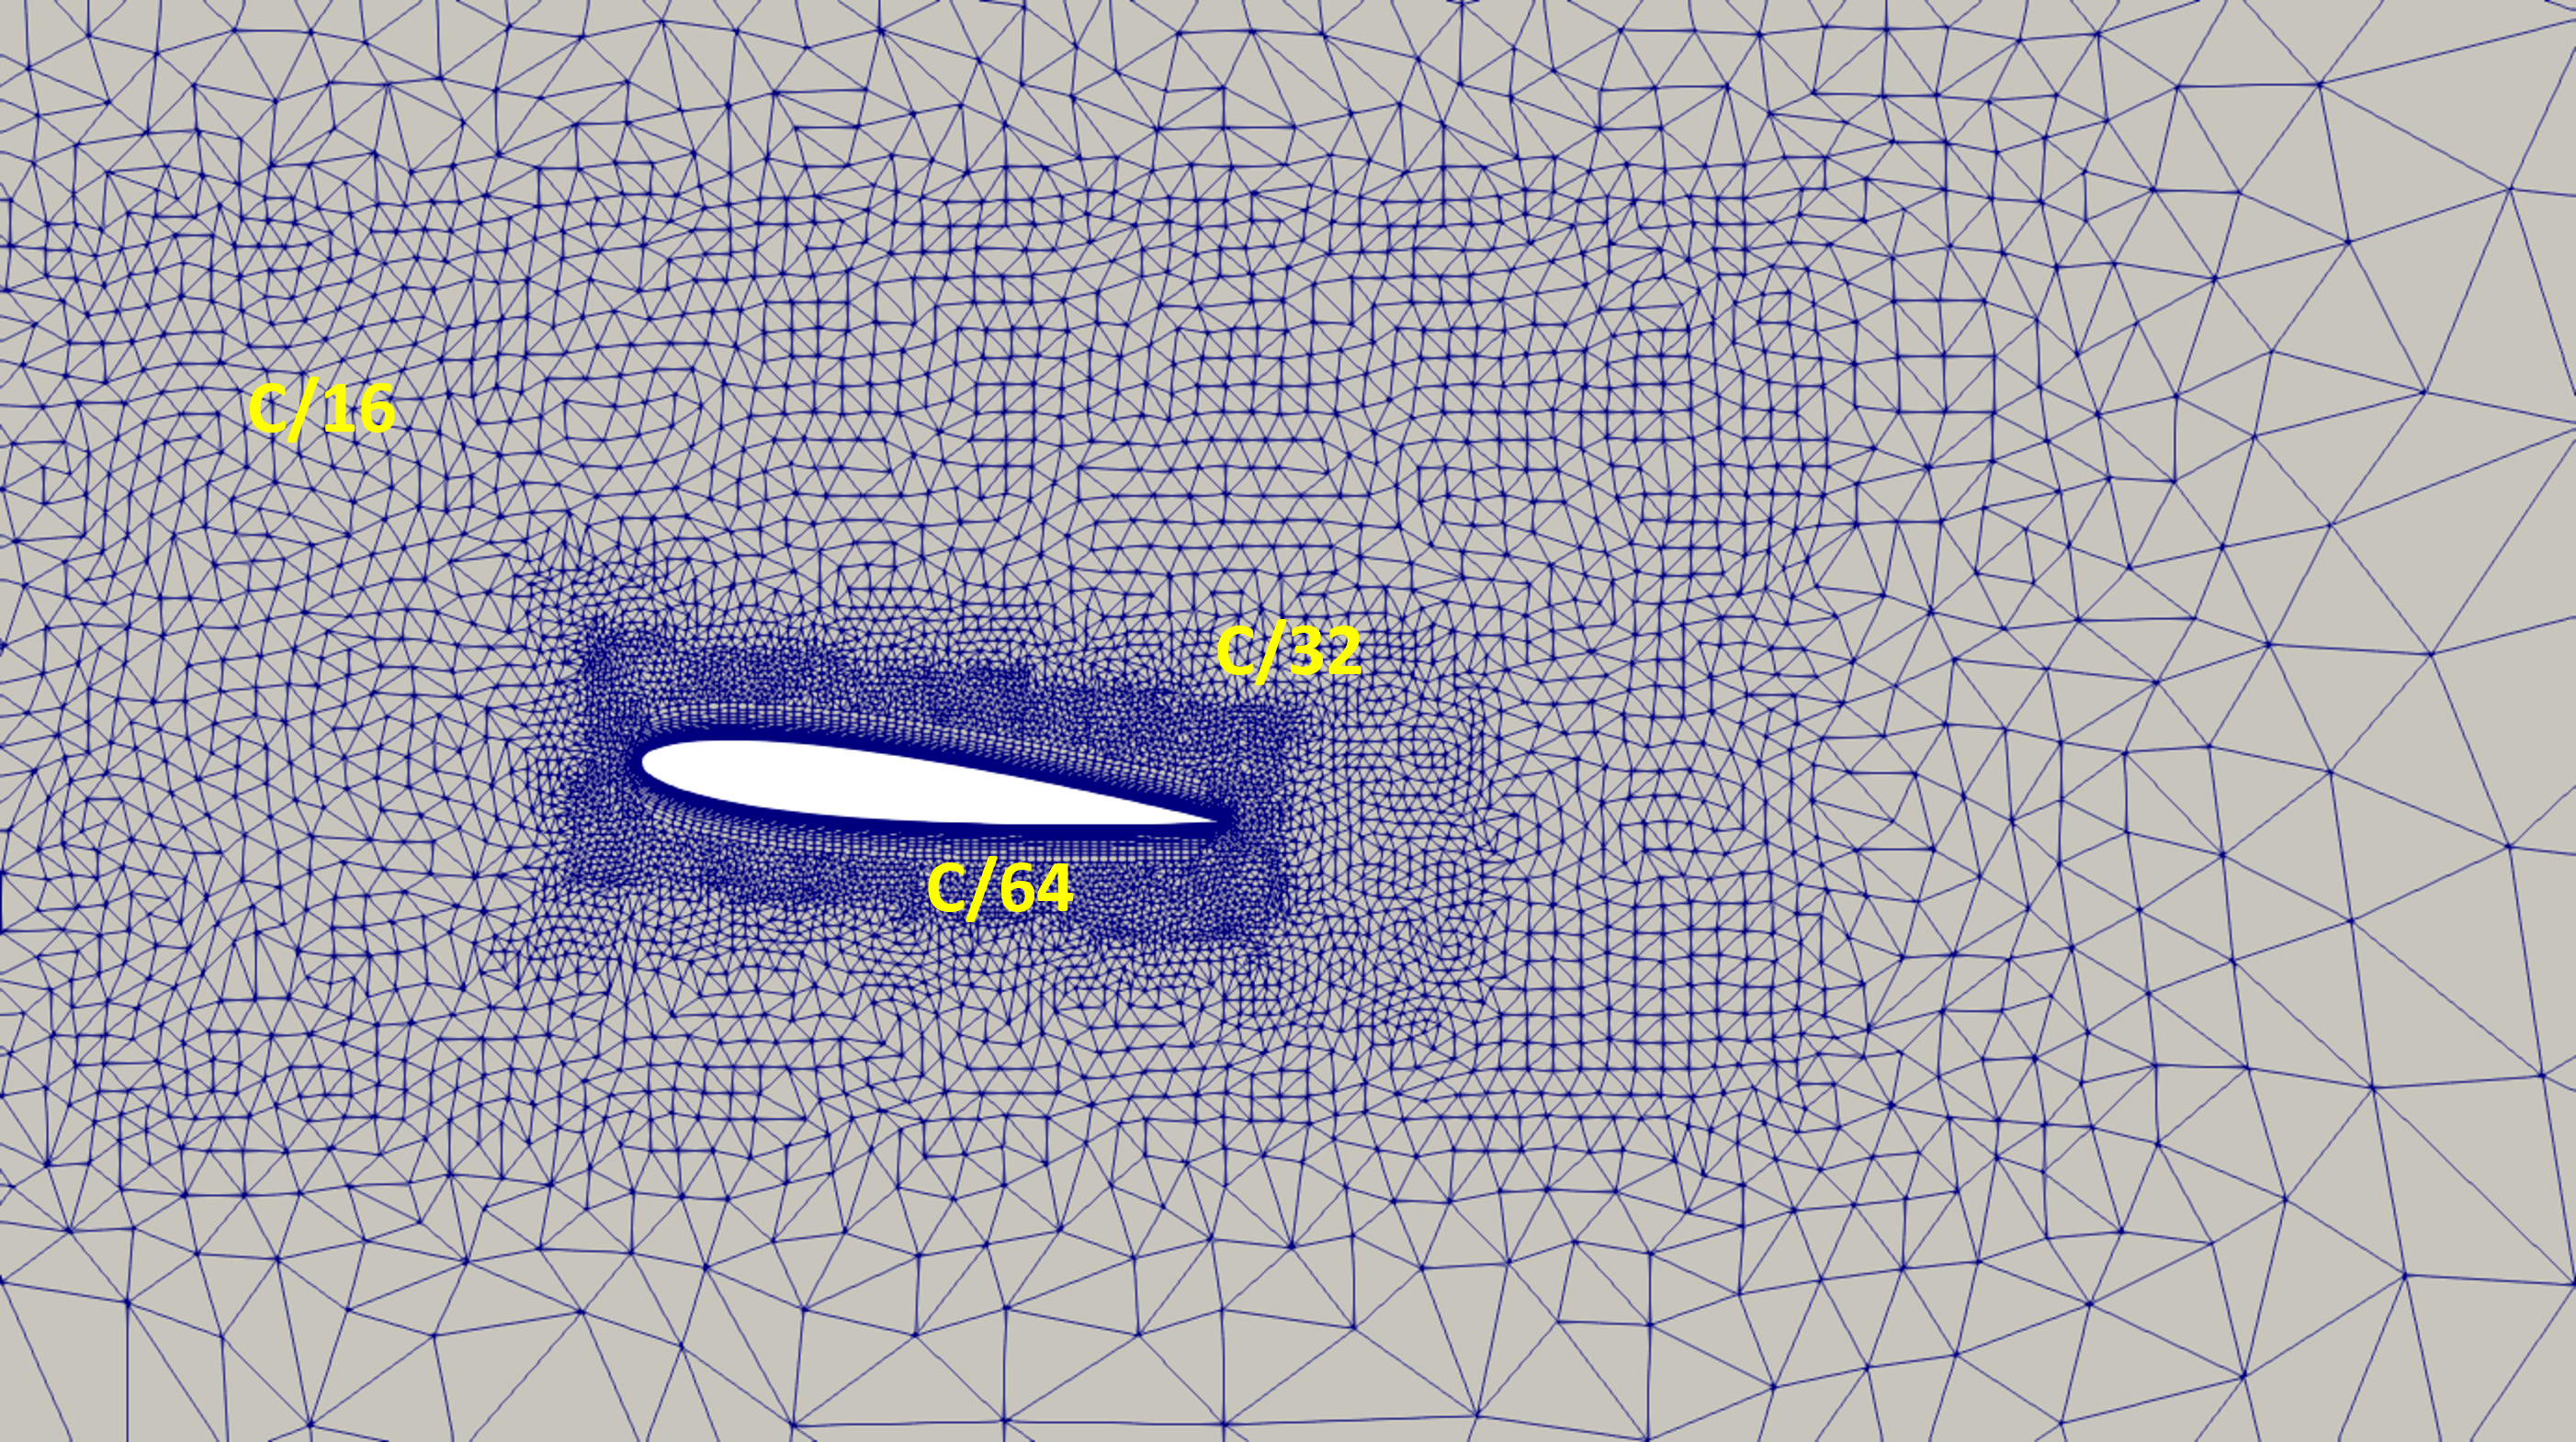
\includegraphics[width=1\textwidth]{figures/adapt_strat/M0_mesh.png}
\caption{M0\_nz25 mesh}
\label{fig:M0_mesh_sa}
\end{subfigure}
\begin{subfigure}[b]{0.475\textwidth}
\centering
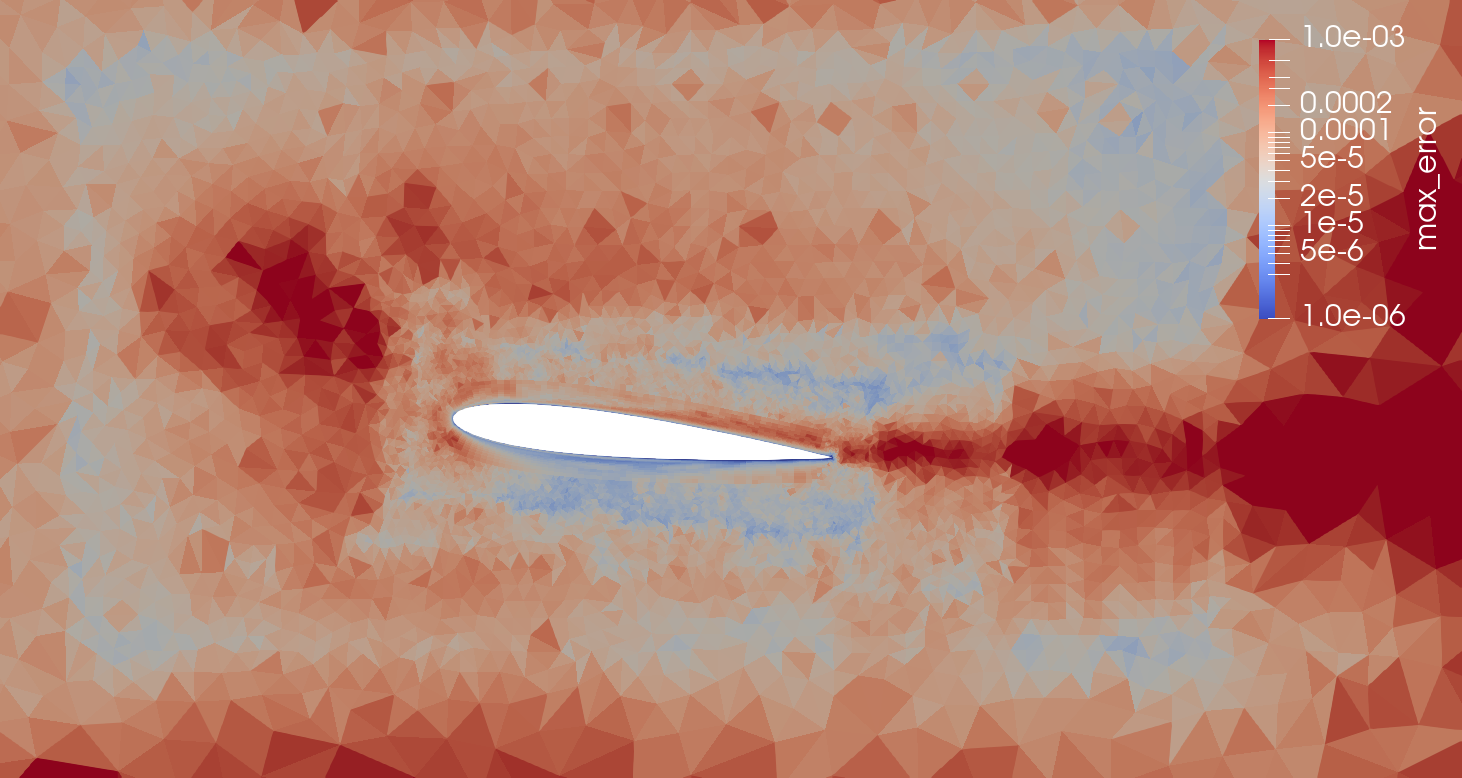
\includegraphics[width=1\textwidth]{figures/adapt_strat/M0_error.png}
\caption{M0\_nz25 error field}
\label{fig:M0_err_plot_sa}
\end{subfigure}
\begin{subfigure}[b]{0.475\textwidth}
\centering
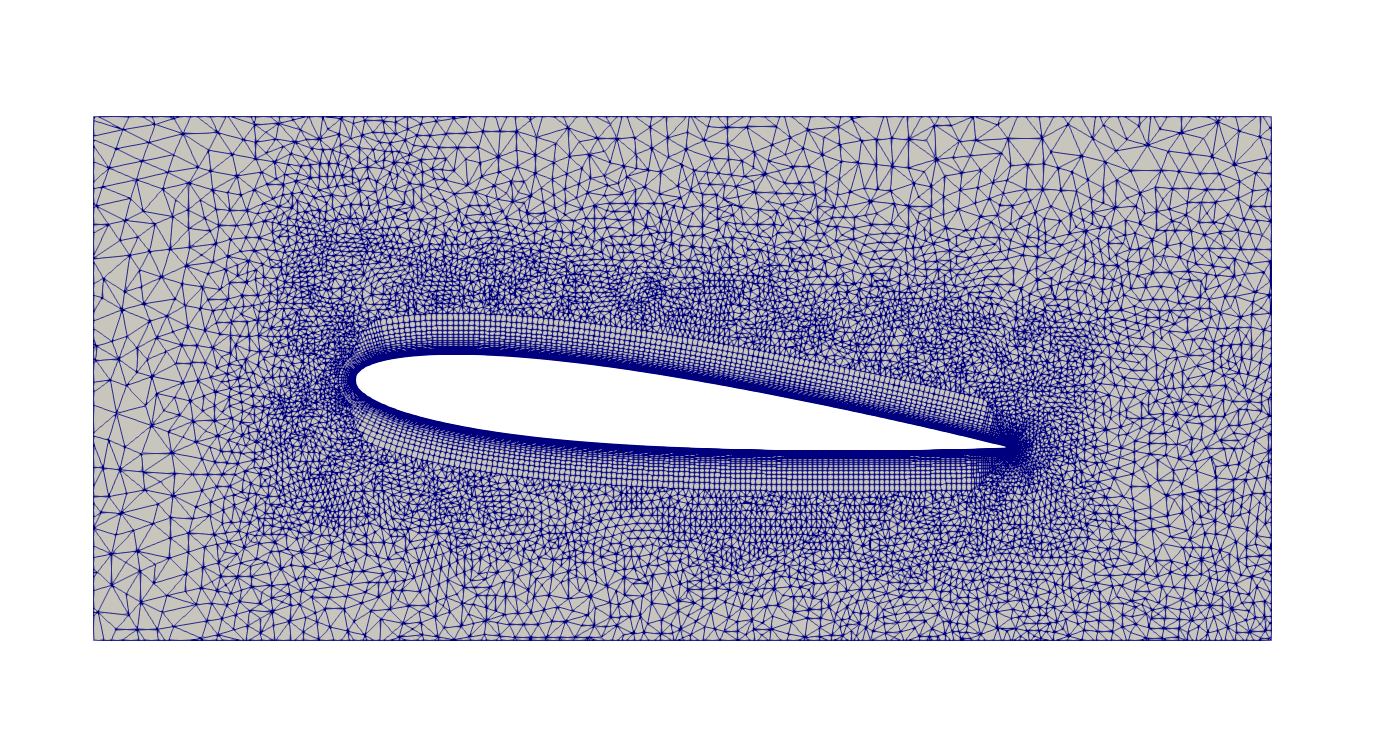
\includegraphics[width=1\textwidth]{figures/adapt_strat/Msa1_mesh.png}
\caption{Msa1\_nz50 mesh}
\label{fig:h_adapt1_mesh}
\end{subfigure}
\begin{subfigure}[b]{0.475\textwidth}
\centering
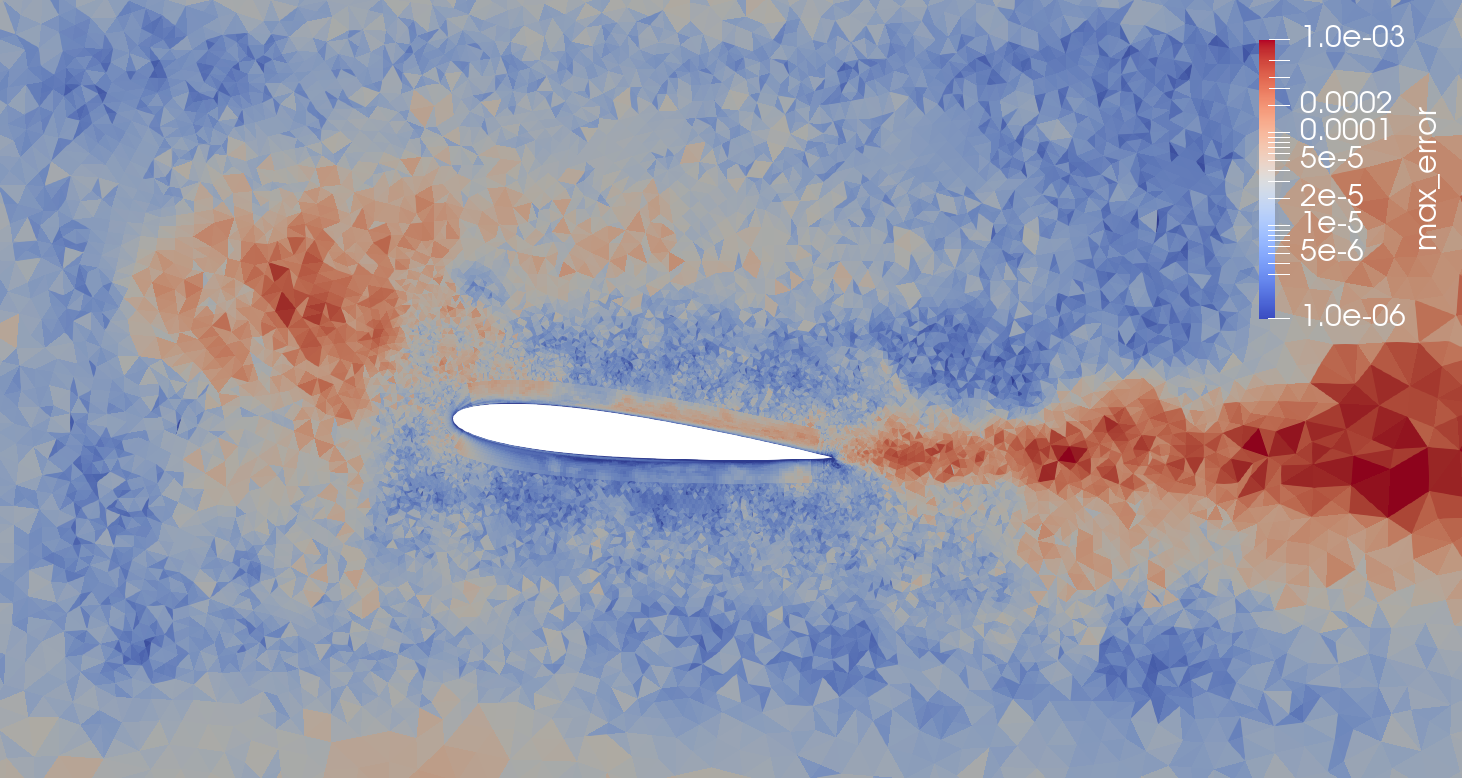
\includegraphics[width=1\textwidth]{figures/adapt_strat/Msa1_error.png}
\caption{Ms\_nz50 error field}
\label{fig:h_adapt1_error_plot}
\end{subfigure}

\caption{Meshes and estimated error fields for size-based strategy}
\end{figure}

As before, M0\_nz25 is used as the initial mesh (Figure \ref{fig:M0_mesh}) and the corresponding error estimated on M0\_nz25 mesh (Figure \ref{fig:M0_err_plot}) is used to calculate nodal size field (i.e., $h_{new}$ at every mesh node/vertex). The mesh adaptation is limited or controlled to have a maximum refinement and maximum coarsening by a factor of 2 to avoid excessive refinement or coarsening in any local region. The number of extruded layers in the spanwise direction are doubled to 50. The adapted mesh obtained using this strategy is shown in Figure \ref{fig:h_adapt1_mesh}. It is referred to as the Msa1\_nz50 mesh (where sa is short for size-based adaptation and 1 in sa1 denotes the first iteration of mesh adaptation). Note that in terms of mesh resolution, this adapted mesh, Msa1\_nz50, compares well against the Mza1\_nz50 mesh obtained from the zonal-based strategy. Msa1\_nz25 mesh consists of 2,859,450 elements, which is comparable to 2,874,300 elements for the Mza1\_n50 mesh. The major differences between the two meshes is that Mza1\_nz50 maintains the same mesh size in various zones, whereas mesh size varies locally (even within a zone) in Msa1\_nz50.
The corresponding estimated error for this mesh is shown in Figure \ref{fig:h_adapt1_error_plot}. Comparing the estimated error between the Msa1\_nz50 and Mza1\_nz50 meshes, higher error values are similarly observed in the LEV regions as well as in the wake of the airfoil. A more detailed comparison of different adaptive strategies/adapted meshes is provided in Section \ref{sec:results_adapt}.
